\documentclass[../main]{subfiles}
\begin{document}

\chapter{Logistic Regression}
\begin{introduction}
\item 
\end{introduction}
\begin{example}
  \textbf{Binary Classification Problem}
\end{example}
Settings.
\begin{itemize}
  \item Dataset: $D=\{(x_i,y_i)\}_{i=1}^n$, where $x_i\in\mathbb{R}^d$ and $y_i\in\{0,1\}$.  
  Here, $y_i$ denotes the classification target, while $x_i$ represents the input features used to predict $y_i$.
  \item Model in Logistic Regression: In logistic regression, we start with a linear model $
  f(x) = w^\top x + b$
  Unlike in ordinary regression, where the target variable lies in $\mathbb{R}$, here the target space collapses to $\{0,1\}$. Thus, we need a function that maps real-valued outputs into this discrete set. Moreover, in many applications it is desirable to obtain not only a hard classification decision (0 or 1), but also a \emph{soft} prediction: the probability of each class. Such a probabilistic interpretation provides both the likelihood estimate and the corresponding classification outcome.
\end{itemize}
Can we directly use a linear model to fit $p(y=1 \mid x=x_i)$, as we did in the previous chapter? The answer is \emph{no}. This is because there is a mismatch between the range of a linear model output (which lies in $\mathbb{R}$) and the valid domain of probabilities, $[0,1]$. 

To resolve this issue, we introduce a transformation function called the \textbf{sigmoid} function. The sigmoid maps any real-valued input into the interval $[0,1]$, making it suitable for modeling probabilities. It is defined as:
\begin{definition}[Sigmoid Function]
  \begin{equation}
    \sigma(z) = \frac{1}{1 + e^{-z}} .
\end{equation}
\end{definition}

\begin{figure}[H]
  \centering
  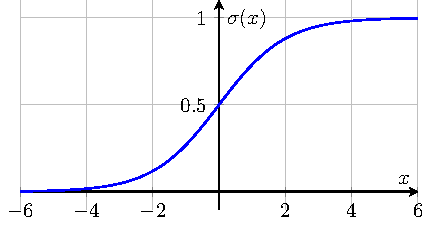
\includegraphics{../../tikz/2/1.pdf}
  \caption{The sigmoid function $\sigma(z)$ over the interval $z \in [-6,6]$.}
\end{figure}

The sigmoid function enjoys several elegant properties.

\begin{theorem}
\[
1 - \sigma(z) = \sigma(-z) .
\]
\end{theorem}

\begin{proof}
This follows directly from the definition of $\sigma(z)$, or equivalently, by observing the symmetry of its graph.
\end{proof}

To convert soft prediction results into binary outputs $\{0,1\}$, we introduce a threshold: when $\sigma(z) = 0.5$, the model makes a hard prediction.

\begin{definition}[Separating Hyperplane]
The condition $\sigma(z) = 0.5$ defines the \emph{separating hyperplane}. It partitions the input space $\mathbb{R}^d$ into two regions, thereby transforming probabilistic predictions into binary classification outcomes.
\end{definition}
The normal vector $w$ is perpendicular to this hyperplane and points towards the region where the model predicts class $1$ 
(i.e., where $p(y=1 \mid x) > 0.5$). 
We ensure this property by choosing the orientation of $w$ accordingly.
\begin{figure}[H]
  \centering
  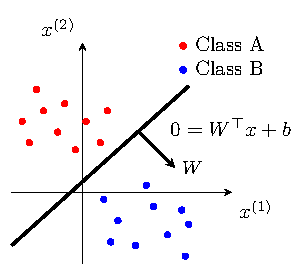
\includegraphics{../../tikz/2/2.pdf}
  \caption{Classification by heperplane.}
  \label{2-lr}
\end{figure}


Model definition is clear, and now we turn our attention to parameter optimization. 
The question is: how can we find the proper $w, b$ that achieve the best performance? 
The key problem here is to identify a suitable loss function that can be optimized via gradient descent.

Notice that:
\begin{equation}
    P(y=1 \mid x = x_i) = \sigma(f(x_i)) = \frac{1}{1+\exp(-w^\top x + b)} .
\end{equation}
We introduce a new method rather than continuing with ERM, by using \textbf{Maximum Likelihood Estimation (MLE)}. 
MLE is naturally designed to address probability modeling problems.

\begin{definition}[Maximum Likelihood Estimation (MLE)]
    MLE aims to find parameters such that the likelihood of $P(y=y_i \mid x=x_i)$ is maximized.
\end{definition}

\begin{remark}
  For brevity, we write $P(y=y_i \mid x=x_i)$ as $P(y_i \mid x_i)$.
\end{remark}
\begin{definition}[Likelihood]
  The likelihood on the entire training data is defined as
  \begin{equation}
      \prod_{i \in [n]} P(y_i \mid x_i; w, b),
  \end{equation}
  assuming the samples are independent.
\end{definition}

According to the discussion above, in logistic regression we have
\begin{equation}
    P(y_i \mid x_i) =
    \begin{cases}
      \sigma(w^\top x_i + b), & y_i = 1, \\
      1 - \sigma(w^\top x_i + b), & y_i = 0.
    \end{cases}
\end{equation}

Therefore, the likelihood function can be expanded as
\begin{equation}
  \prod_{i \in [n]} \sigma(w^\top x_i + b)^{y_i} \,
  \big(1 - \sigma(w^\top x_i + b)\big)^{1-y_i}
\end{equation}

The above form is intuitive once we recall that $x^0 = 1$.

To ensure floating-point precision, given the large amount of data and the monotonicity of the logarithm function, 
we transform the likelihood into the maximization of the log-likelihood:
\begin{equation}
    \argmax_{w,b} \sum_{i \in [n]} 
    \Big[ y_i \log \sigma(w^\top x_i + b) 
    + (1-y_i) \log \big(1 - \sigma(w^\top x_i + b)\big) \Big]
\end{equation}
This is the final objective in MLE.

MLE can be transformed into ERM by applying $\argmin$ to the negative log-likelihood. 
Thus we define the \textbf{Cross-entropy Loss}:
\begin{equation}
    \mathcal{L}(w,b) 
    := - \sum_{i \in [n]} \Big[ 
      y_i \log \sigma(w^\top x_i + b) 
      + (1-y_i) \log \big(1 - \sigma(w^\top x_i + b)\big) 
    \Big]
\end{equation}
\begin{note}
  Why is the above loss called the {Cross-entropy loss}? 
  The name originates from information theory. 
  Entropy is defined as:
  \begin{equation}
      H(P) = \sum_y P(y)\log\frac{1}{P(y)} 
           = -\sum_y P(y)\log P(y).
  \end{equation}
  In other words, rarer events (with smaller probability) carry more information, 
  and entropy measures the expected amount of information. In our context, we can evaluate the information content of the prediction 
  for $y = \hat y_i$ given $x = x_i$ as:
  \begin{align}
      H(P) &= - \sum_{\hat y_i \in \{0,1\}} 
      P(y=\hat y_i \mid x_i)\,\log P(y=\hat y_i \mid x_i)\notag\\
      &=-[P(y=1\mid x_i)\,\log P(y=1\mid x_i)+P(y=0 \mid x_i)\,\log P(y=0 \mid x_i)]
  \end{align}
  Notice that $P(y=1 \mid x_i) = \sigma(f(x_i; w,b))$ and $P(y=0 \mid x_i) = 1 - \sigma(f(x_i; w,b))$. In practice, we substitute the empirical distribution of samples for the true distribution when comparing the negative log-likelihood with entropy. This is why the terminology of entropy from information theory is carried over to name this loss term.
\end{note}
\begin{note}
  The formal definition of cross entropy between two propbability distributions $q$ and $p$ $H(q,p)$ is defined by:
  \begin{equation}
      H(q,p)=-\sum_y q(y)\log p(y)
  \end{equation}
\end{note}
\begin{definition}[KL-Divergence]
  The KL-Divergence between two distributions $p$ and $q$ is defined by:
    \begin{equation}
        \mathrm{KL}(q\Vert p)=\sum_y q(y)\log\frac{q(y)}{p(y)}
    \end{equation}
\end{definition}
KL-Divergence measures the difference between two given distributions. 
In particular, $\mathrm{KL}(q \Vert p)$ differs from the cross-entropy by only a constant term $H(q)$:
\begin{equation}
  \mathrm{KL}(q \Vert p) = H(q, p) - H(q).
\end{equation}
In other words, KL-Divergence quantifies the extra number of bits required when we use $p$ to approximate the ground-truth distribution $q$.

\vspace{1em}
Back to the main content. Rewind that closed-form solution can be extract from linear regression problem as we mensioned in last chapter, we hope to find out whether logistic regression has closed form solution.

Following the same steps we applied in linear case, we define $\hat x=(x^\top,1)^\top\in\mathbb R^{d+1}$ and $\hat w=(w^\top,b)^{\top}\in\mathbb R^{d+1}$, thus $f(x)=\hat w^\top \hat x$:
\begin{align}
  \mathcal L(\hat w)&=-\sum_{i\in[n]}y_i\log\sigma(\hat w\hat x_i)+(1-y_i)\log(1-\sigma(\hat w^\top\hat x_i))\notag\\
  &=-\sum_{i\in[n]}y_i\log\frac{1+\exp(\hat w^\top\hat x_i)}{1+\exp(-\hat w^\top\hat x_i)}-\log(1+\exp(\hat w^\top\hat x_i))\notag\\
  &=-\sum_{i\in[n]}y_i(\hat w^\top\hat x_i)-\log(1+\exp(\hat w^\top\hat x_i))
\end{align}
Dereviate:
\begin{align}
  \frac{\partial\mathcal L(\hat w)}{\partial \hat w}&=-\sum_{i\in[n]}\left[y_i\hat x_i-\frac{\exp(\hat w^\top\hat x_i)}{1+\exp(\hat w^\top\hat x_i)}\hat x_i\right]\\
  &=-\sum_{i\in [n]}\left[y_i-P(y=1\mid x_i)\right]\hat x_i
\end{align}
By gradient descent, the parameter is updated as$
  \hat w \;\leftarrow\; \hat w + \alpha \sum_{i \in [n]} \Big(y_i - P(y_i=1 \mid x_i)\Big)\,\hat x_i .$
This makes sense, since the term $y_i - P(y_i=1 \mid x_i)$ directly measures the prediction error on sample $i$, and the update moves $\hat w$ a small step along the direction of the input $\hat x_i$ to reduce this error.

If for all $i$, we have $y_i = P(y=1 \mid x_i)$, then the model predicts every label $y_i$ perfectly. At this point, optimization reaches a stationary solution. If the training data admits such a perfect solution, that is, if all points can be separated by a linear model without error, we say the dataset is \textbf{linearly separable}.

Example \ref{2-lr} is linearly separable, and the final state leads to $\|W\| \to \infty, \quad \|b\| \to \infty$. However, this situation is not desirable in practice, since it implies poor robustness. Hence a natural question arises: under the condition of linear separability, how can we find a well-chosen separating hyperplane that maximizes robustness? The answer will be presented in the next chapter, where we introduce the Support Vector Machine (SVM). The SVM optimizes $\hat w, \hat b$ by maximizing the margin (the distance between data points and the separating hyperplane), instead of simply minimizing the cross-entropy loss.

Although logistic regression may suffer from divergence of parameters under separable data, it often achieves better performance than SVM in practice, due to the following reasons:
\begin{enumerate}
  \item In most real-world problems, the data are not linearly separable;
  \item Applying $L_2$ regularization can effectively prevent parameter divergence.
\end{enumerate}
\begin{remark}
  Why can't we use squared loss for classification? The reason is that in classification tasks such as logistic regression, the label $y \in \{0,1\}$ should be interpreted as a categorical outcome rather than a numerical quantity. 
\end{remark}
\end{document}